% Drawing 154/07-17 -- folder 154, batch 07, archive page 122 (PDF page 123).
% Transcription: à gauche, un disque bordé de jaune, deux points marqués sur le bord, contenant une courbe rouge qui se recoupe plusieurs fois ; à côté, le mot « \emph{Non} » (souligné). À droite, des croquis au crayon : un cercle traversé d'une courbe, des droites qui se croisent en étoile sur une droite, des arcs
% Kind: disk with a self-crossing curve, marked « Non »; pencil sketches. Method 2 (schematic redraw from the facsimile). Status: partial.
% Notes: Disk: yellow rim, a black point at the left and at the right of the rim, a red curve entering at the top, winding through three loops and leaving at the bottom; the word « Non », underlined. The curve is followed loosely: its loops are there, the exact number and order of its self-crossings are not reliable. Pencil, right and below: a circle with a curve down through it and two points on its rim; a line carrying two small stars of strokes; below, a long line with an inverted V, a small crossing, a star of six strokes, a second inverted V and a fan of strokes at its right end. The fainter pencil strokes of the upper right are left out. Redrawn 2026-11-12 (issue 128): to check again.
% Coordinates: 1 unit = 1 mm = 1/100 of the crop width (bbox in page fractions: [0.17, 0.09, 0.87, 0.4]).
% Redrawn by Claude (claude-fable-5-2), issue #128, 2026-11-12; not checked by a human; not compiled (no TeX in the session).
% Rights: reproduces part of the work -- behind RENDER_TRANSCRIPTS, never published by itself.
\documentclass[tikz,border=3pt]{standalone}
\usepackage{amsmath,amssymb}
\usetikzlibrary{patterns,arrows.meta}
\tikzset{Ye/.style={yellow!80!orange}, Rd/.style={red!85!black}, pencil/.style={black!45}, struck/.style={black!35}, mpt/.style={circle,draw,inner sep=1.3pt}, pt/.style={circle,fill,inner sep=0.9pt}, opt/.style={circle,draw,fill=white,inner sep=1.1pt}}
\begin{document}
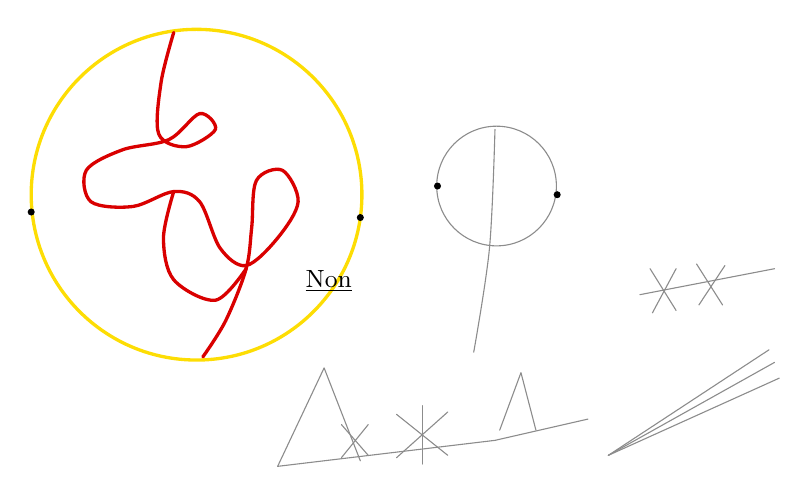
\begin{tikzpicture}[x=1mm,y=1mm,line cap=round,line join=round,font=\scriptsize]
\draw[Ye,very thick] (23.6,-24) circle[radius=21];
\node[pt] at (2.6,-26.2) {};
\node[pt] at (44.4,-26.9) {};
\draw[Rd,very thick] plot[smooth, tension=0.55] coordinates {(20.7,-3.4) (19.1,-9.7) (18.8,-16.3) (22.3,-17.9) (26,-15.7) (24,-13.7) (20.1,-17) (14.2,-18.3) (9.6,-20.9) (10.2,-24.9) (15.5,-25.5) (20.7,-23.6) (24,-24.9) (26.6,-30.8) (29.9,-33) (33.9,-29.5) (36.5,-24.9) (34.5,-20.9) (31.2,-22.2) (30.6,-28.2) (29.9,-33.4) (27.3,-40) (24.4,-44.6)};
\draw[Rd,very thick] plot[smooth, tension=0.55] coordinates {(20.7,-23.6) (19.4,-29.5) (20.7,-34.8) (26,-37.4) (29.9,-33.4)};
\node[inner sep=1pt] at (40.4,-35) {\small \underline{Non}};
\draw[pencil] (61.7,-22.9) circle[radius=7.6];
\draw[pencil] plot[smooth, tension=0.55] coordinates {(61.5,-15.7) (60.8,-30.8) (58.8,-44)};
\node[pt] at (54.2,-22.9) {};
\node[pt] at (69.4,-24) {};
\draw[pencil] (79.9,-36.7) -- (97,-33.4);
\draw[pencil] (81.2,-33.4) -- (84.5,-38.7);
\draw[pencil] (84.5,-33.4) -- (81.5,-39);
\draw[pencil] (87.1,-32.8) -- (90.4,-38);
\draw[pencil] (90.7,-33) -- (87.4,-38);
\draw[pencil] (33.9,-58.5) -- (61.5,-55.2) -- (73.3,-52.5);
\draw[pencil] (33.9,-58.5) -- (39.8,-46) -- (44.4,-57.8);
\draw[pencil] (42,-53.2) -- (45.4,-57.1);
\draw[pencil] (45.4,-53.2) -- (42,-57.4);
\draw[pencil] (49,-51.9) -- (55.5,-57.1);
\draw[pencil] (55.5,-51.6) -- (49,-57.4);
\draw[pencil] (52.3,-50.8) -- (52.3,-58.2);
\draw[pencil] (62.1,-53.9) -- (64.8,-46.6) -- (66.7,-53.9);
\draw[pencil] (75.9,-57.1) -- (97,-45.3);
\draw[pencil] (75.9,-57.1) -- (97.6,-47.3);
\draw[pencil] (75.9,-57.1) -- (96.3,-43.7);
\end{tikzpicture}
\end{document}
